\documentclass[a4paper]{article}

\usepackage[UTF8]{ctex}
\usepackage[a4paper,margin=1in]{geometry}
\usepackage{graphicx}
\usepackage{float}
\usepackage{listings}
\usepackage{longtable}
\usepackage{booktabs}
\usepackage{hyperref}
\usepackage{fancyhdr}
\usepackage{lastpage}
\usepackage{color}
\usepackage{xcolor}
\usepackage{indentfirst}        % 首段缩进
\setlength{\parindent}{2em}     % 缩进2字符
\usepackage{zhnumber}           % 中文编号
\usepackage[dvipsnames]{xcolor}
\usepackage{amsmath}
\usepackage{multimedia}  % 添加多媒体支持
\usepackage{qrcode}      % 添加二维码支持(可选)
\usepackage[most]{tcolorbox}  % 添加彩色框支持
%\newcommand{\college}{中山大学计算机学院}
\newcommand{\projname}{计算机图形学|作业二}
\newcommand{\reporttitle}{三角形光栅化与着色算法实验}
\newcommand{\stuno}{23336179}
\newcommand{\authorname}{马福泉}
\newcommand{\major}{计算机科学与技术}
\newcommand{\adviser}{陶钧}
\newcommand{\startdate}{2025年11月25日}
\newcommand{\labenddate}{2025年12月2日}
\newcommand{\labroom}{B402}

\pagestyle{fancy} % 使用 fancyhdr 风格
\fancyhf{}      % 清空默认的页眉页脚

% 设置页眉
\fancyhead[L]{\kaishu \projname}      % 左侧页眉显示项目名称
\fancyhead[C]{\kaishu \reporttitle}    % 中间页眉显示报告标题
\fancyhead[R]{\kaishu \authorname} % 右侧页眉显示作者姓名

% 设置页脚
\fancyfoot[C]{第 \thepage 页，共 \pageref{LastPage} 页} % 中间页脚显示页码

% 去除页眉页脚与正文之间的分隔线
\renewcommand{\headrulewidth}{0.4pt}
\renewcommand{\footrulewidth}{0pt}

% 设置文档背景颜色
\definecolor{mybgcolor}{RGB}{0, 0, 0} % 定义背景颜色
\definecolor{NavyBlue}{RGB}{0,0,128} % 添加颜色定义
% \pagecolor{mybgcolor} % 设置背景颜色

\lstset{
    basicstyle=\ttfamily\small,
    commentstyle=\color{gray},
    keywordstyle=\color{blue},
    stringstyle=\color{red},
    breaklines=true,
    frame=single,
    numbers=left,
    numberstyle=\tiny\color{gray},
    tabsize=4,
    showstringspaces=false,
    captionpos=b,
    language=C++
}

\begin{document}

% 封面
\begin{titlepage}
    \centering
    

    
\includegraphics[width=10cm]{img/SYSULogo.png}

    \vspace{1em}
    %{\Large \college \par}
    \vspace{1em}
    {\Large \kaishu \projname \par}
    \vspace{3em}

    

    
    {\fontsize{40pt}{42pt}\kaishu \selectfont \boldmath \reporttitle\par}
    \vspace*{\fill}

    \begin{center}
    {\Large
    \makebox[5em][s]{学号}:\underline{\makebox[15em][c]{\kaishu \stuno}}\\[1em]
    \makebox[5em][s]{姓名}:\underline{\makebox[15em][c]{\kaishu \authorname}}\\[1em]
    \makebox[5em][s]{专业}:\underline{\makebox[15em][c]{\kaishu \major}}\\[1em]
    \makebox[5em][s]{课程教师}:\underline{\makebox[15em][c]{\kaishu \adviser}}\\[1em]
    \makebox[5em][s]{起始日期}:\underline{\makebox[15em][c]{\kaishu \startdate}}\\[1em]
    \makebox[5em][s]{结束日期}:\underline{\makebox[15em][c]{\kaishu \labenddate}}\\[1em]
    \makebox[5em][s]{实验地点}:\underline{\makebox[15em][c]{\kaishu \labroom}}
    }
    \end{center}

    \vspace*{\fill}
\end{titlepage}

% 目录
\tableofcontents
\newpage

% 实验报告正文开始

\section{实验概述}

本次计算机图形学作业二主要包含两个核心实验：三角形光栅化算法实现和光照着色算法实现。通过这两个实验，深入理解图形学中基础的几何图元绘制和光照模型的原理与应用。

\subsection{三角形光栅化算法}

\textbf{实验要求：}

\begin{enumerate}
\item[\textbf{1.1}] 用DDA算法实现三角形边的绘制
\item[\textbf{1.2}] （选做）用Bresenham算法实现三角形边的绘制  
\item[\textbf{1.3}] 用edge-walking算法填充三角形内部颜色
\item[\textbf{1.4}] 针对不同面数的模型，从实际运行时间角度讨论不同算法的绘制效率
\end{enumerate}

\textbf{性能测试提示：}

可以使用\texttt{glfwGetTime()}函数进行时间测量：
\begin{lstlisting}
double startTime = glfwGetTime();  // 开始计时（时间戳）
double endTime = glfwGetTime();    // 结束计时（时间戳）
renderTimeMs = (float)((endTime - startTime) * 1000.0);  // 渲染时间（ms）
\end{lstlisting}

\subsection{光照着色算法}

\textbf{实验要求：}

\begin{enumerate}
\item[\textbf{2.1}] 用Gouraud模型实现三角形内部的着色
\item[\textbf{2.2}] （选做）用Phong模型实现三角形内部的着色
\item[\textbf{2.3}] （选做）用Blinn-Phong模型实现三角形内部的着色  
\item[\textbf{2.4}] 结合实际运行时间讨论不同着色方法的效果、着色效率
\end{enumerate}

\subsection{最终效果展示}

\begin{enumerate}
\item[\textbf{3.1}] 对于第1题，加载单一三角形情况下，程序界面提供了“DDA”和“Bresenham”两种算法的切换选项。可以通过勾选不同的单选框（Radio Button）来实时切换边缘绘制算法，并观察展示DDA-EdgeWalking或Bresenham-EdgeWalking的三角形光栅化效果是否正确。

\item[\textbf{3.2}] 对于第2题，程序支持加载正方体、正四面体等不同面数的模型。在Control Panel中提供了“Flat”、“Gouraud”、“Phong”和“Blinn-Phong”四种着色模式的切换选项。可以通过勾选不同的单选框来实时切换着色算法，并观察不同模型在不同着色模式下的光照效果差异。并通过光照模型公式和材质参数共同决定环境光、散射光（漫反射）、高光（镜面反射）效果的呈现。
\end{enumerate}

\section{实现过程}

\subsection{环境准备}

本次实验在作业1的GLFW+ImGUI环境基础上，引入了GLM库（OpenGL Mathematics）。GLM是一个专门为图形学设计的数学库，提供了向量和矩阵运算支持。

\subsubsection{引入GLM库}

\textbf{前期准备：}
基于作业1已配置好的GLFW+ImGUI环境，在项目根目录下新建 \texttt{include} 文件夹，并将解压后的 \texttt{glm} 文件夹放入其中。目录结构如下：
\begin{verbatim}
项目文件夹/
  |-- CMakeLists.txt
  |-- main.cpp
  +-- include/
       +-- glm/
            |-- glm.hpp
            +-- ...
\end{verbatim}

\textbf{修改CMakeLists.txt：}
在原有的 \texttt{CMakeLists.txt} 中，找到 \texttt{target\_include\_directories} 部分，添加 \texttt{include} 目录的引用：

\begin{lstlisting}[language=bash]
target_include_directories(${PROJECT_NAME} PRIVATE
    ${imgui_SOURCE_DIR}
    ${imgui_SOURCE_DIR}/backends
)
# 新增下面这一行
include_directories("${CMAKE_SOURCE_DIR}/include")
\end{lstlisting}

\textbf{重置构建缓存：}
由于项目结构发生变化，在Visual Studio中打开项目后，执行“项目” -> “删除缓存并重新配置” (Delete Cache and Reconfigure)，等待CMake重新生成构建文件。

\subsubsection{环境测试}

为了验证GLM库是否成功引入，编写了测试代码进行矩阵变换测试。

运行结果如下图所示，GLM库工作正常：
\begin{figure}[H]
    \centering
    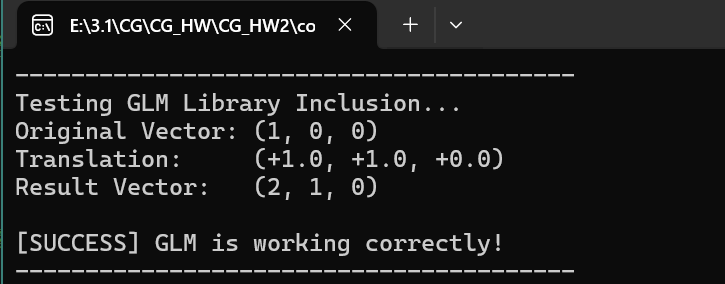
\includegraphics[width=0.8\textwidth]{img/set_success.png}
    \caption{GLM库环境配置测试成功截图}
    \label{fig:env_test}
\end{figure}

\subsection{三角形的光栅化}

\subsubsection{算法原理}
\begin{itemize}
    \item \textbf{DDA算法}：数字微分分析仪（Digital Differential Analyzer）是一种基于直线的微分方程来生成直线的算法。它利用浮点数增量计算，通过计算斜率 $k = \Delta y / \Delta x$，每次 $y$ 增加1时，$x$ 增加 $1/k$（对于 $y$ 主轴）。
    \item \textbf{Bresenham算法}：一种高效的整数增量算法。它通过维护一个误差项 $d$，根据误差项的符号决定下一个像素点的选择，避免了浮点运算和除法，适合硬件实现。
    \item \textbf{Edge-Walking（扫描线算法）}：用于填充多边形内部。算法首先将多边形的顶点按 $y$ 坐标排序，然后从上到下逐行扫描。对于每一行扫描线，计算其与多边形边的交点（左右边界），并填充这两个交点之间的像素。
\end{itemize}

\subsubsection{实现思路}
在 \texttt{main.cpp} 中定义了 \texttt{RasterizeTriangle\_DDA} 和 \texttt{RasterizeTriangle\_Bresenham} 两个函数。
\begin{enumerate}
    \item \textbf{顶点排序}：首先将三角形的三个顶点按 $y$ 坐标从小到大排序 ($p_0, p_1, p_2$)。
    \item \textbf{三角形分割}：将三角形分为上半部分（$p_0-p_1$ 高度）和下半部分（$p_1-p_2$ 高度）。长边始终是 $p_0-p_2$。
    \item \textbf{边界计算}：
    \begin{itemize}
        \item 对于 DDA，直接利用浮点数插值计算每一行 $y$ 对应的左右边界 $x$ 坐标以及属性（深度、法线、颜色等）。
        \item 对于 Bresenham，实现了一个 \texttt{BresenhamWalker} 结构体，利用整数运算迭代更新 $x$ 坐标。
    \end{itemize}
    \item \textbf{扫描线填充}：在计算出左右边界 $[x_{left}, x_{right}]$ 后，对区间内的每个像素进行深度测试和着色计算。
\end{enumerate}

\subsubsection{核心代码}

\textbf{DDA 光栅化核心逻辑：}
\begin{lstlisting}
// 左右边缘遍历器，利用 Lerp 插值属性
for (int i = 0; i < totalHeight; ++i) {
    // ... 计算 t_long, t_short ...
    Attribs attr_long = Attribs::Lerp(a0, a2, t_long);
    Attribs attr_short = Attribs::Lerp(a0, a1, t_short); 

    // ...
    
    // 扫描线填充
    for (int x = xl; x <= xr; x++) {
        float t_span = (spanWidth == 0) ? 0 : (float)(x - xl) / spanWidth;
        Attribs frag = Attribs::Lerp(attr_long, attr_short, t_span);
        // 深度测试与着色 
        SetPixel(x, y, frag.z, finalColor);
    }
}
\end{lstlisting}

\textbf{Bresenham 辅助类：}
\begin{lstlisting}
struct BresenhamWalker {
    int x, dx, totalY, sx, rem;
    void InitIntDDA(glm::vec3 start, glm::vec3 end) {
        // 初始化 dx, totalY, sx
        rem = 0;
    }
    void Step() {
        if (totalY == 0) return;
        int inc = dx / totalY;
        x += inc * sx;
        rem += (dx % totalY);
        if (rem >= totalY) {
            x += sx;
            rem -= totalY;
        }
    }
};
\end{lstlisting}

\subsubsection{结果展示}
\begin{figure}[H]
    \centering
    \begin{minipage}[t]{0.48\textwidth}
        \centering
        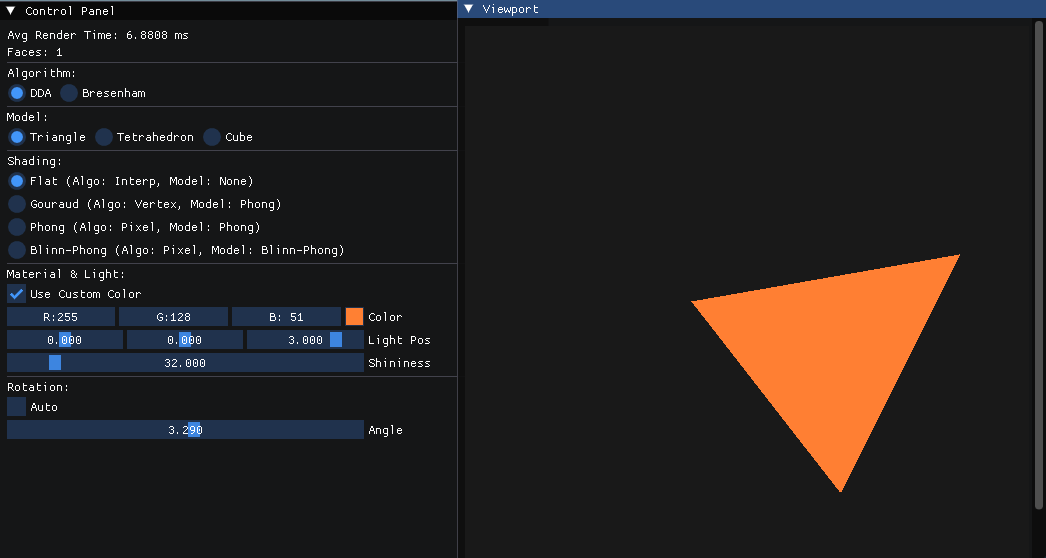
\includegraphics[width=\textwidth]{img/placeholder_dda.png}
        \caption{DDA 算法绘制三角形}
    \end{minipage}
    \begin{minipage}[t]{0.48\textwidth}
        \centering
        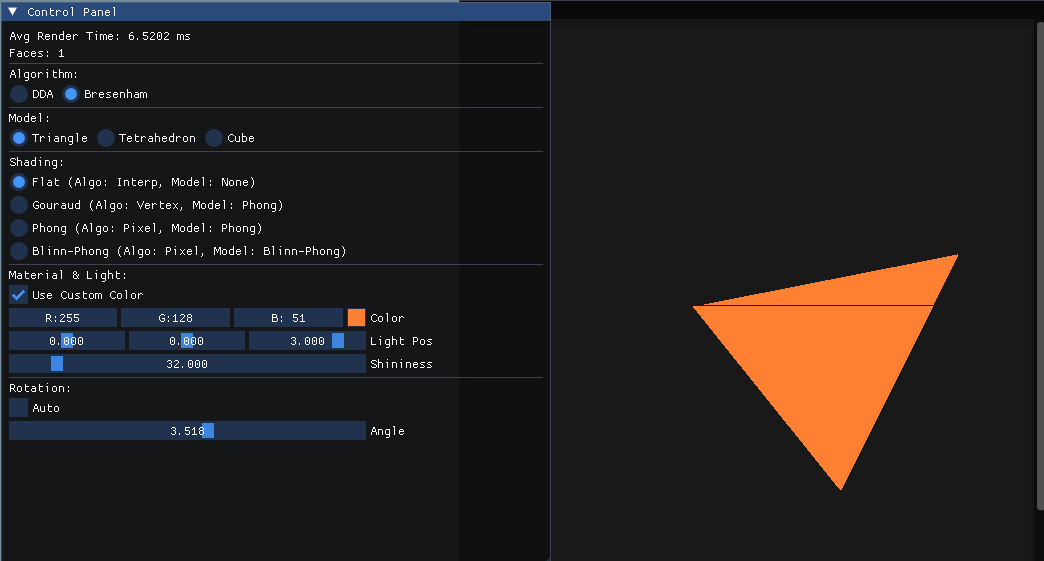
\includegraphics[width=\textwidth]{img/placeholder_bresenham.png}
        \caption{Bresenham 算法绘制三角形}
    \end{minipage}
\end{figure}

\subsection{着色实验和光照模型}

本实验实现了三种主要的着色方案，分别对应不同的着色频率（Shading Frequency）和光照模型（Lighting Model）。

\subsubsection{Gouraud Shading (Algo: Vertex, Model: Phong)}

\textbf{原理与特点：}
Gouraud着色是一种\textbf{逐顶点（Per-Vertex）}的着色方法。它在顶点处理阶段，利用Phong光照模型计算每个顶点的颜色。在光栅化阶段，这些顶点颜色被线性插值到三角形内部的每一个片元。
\begin{itemize}
    \item \textbf{优点}：计算量小，效率高。光照计算次数等于顶点数。
    \item \textbf{缺点}：高光效果依赖于网格密度。如果高光位于三角形内部，插值会导致高光丢失或形状失真（Mach bands效应）。
\end{itemize}

\subsubsection{Phong Shading (Algo: Pixel, Model: Phong)}

\textbf{原理与特点：}
Phong着色是一种\textbf{逐片元（Per-Pixel）}的着色方法。它在光栅化阶段对顶点的法向量和世界坐标进行插值，得到每个片元的法向量和位置。然后对每一个片元，使用Phong光照模型计算颜色。
Phong光照模型的高光项计算依赖于反射向量 $R$ 和视线向量 $V$ 的夹角：$I_{spec} = k_s (R \cdot V)^\alpha$。
\begin{itemize}
    \item \textbf{优点}：能够精确表现物体表面的高光，光照效果平滑逼真。
    \item \textbf{缺点}：计算量大，光照计算次数等于屏幕像素数。计算反射向量 $R$ 需要昂贵的数学运算。
\end{itemize}

\subsubsection{Blinn-Phong Shading (Algo: Pixel, Model: Blinn-Phong)}

\textbf{原理与特点：}
Blinn-Phong着色同样是\textbf{逐片元}计算，但采用了Blinn-Phong光照模型。
它对Phong模型的高光计算进行了改进，使用半程向量 $H = \frac{L + V}{|L + V|}$ 与法向量 $N$ 的夹角来近似高光：$I_{spec} = k_s (N \cdot H)^\alpha$。
\begin{itemize}
    \item \textbf{特点}：当视线与光源在表面同一侧时，Blinn-Phong比Phong更高效（避免了反射向量计算）。高光形状通常比Phong略微拉长且边缘更柔和，被认为更符合真实物理规律（微表面理论）。
\end{itemize}

\subsubsection{核心代码实现}

为了支持上述三种模式，核心光照函数 \texttt{CalculateLighting} 实现了两种光照模型，而光栅化循环根据当前模式决定是在顶点处调用还是在片元处调用。

\textbf{光照计算函数：}
\begin{lstlisting}
glm::vec3 CalculateLighting(glm::vec3 fragPos, glm::vec3 normal, glm::vec3 objectColor, bool isBlinn) {
    // 环境光
    glm::vec3 ambient = ambientStrength * lightColor;
    // 漫反射
    glm::vec3 norm = glm::normalize(normal);
    glm::vec3 lightDir = glm::normalize(lightPos - fragPos);
    float diff = std::max(glm::dot(norm, lightDir), 0.0f);
    glm::vec3 diffuse = diff * lightColor;
    // 镜面反射
    glm::vec3 viewDir = glm::normalize(viewPos - fragPos);
    float spec = 0.0f;
    if (isBlinn) { // Blinn-Phong
        glm::vec3 halfwayDir = glm::normalize(lightDir + viewDir);
        spec = std::pow(std::max(glm::dot(norm, halfwayDir), 0.0f), shininess);
    } else { // Phong
        glm::vec3 reflectDir = glm::reflect(-lightDir, norm);
        spec = std::pow(std::max(glm::dot(viewDir, reflectDir), 0.0f), shininess);
    }
    glm::vec3 specular = specularStrength * spec * lightColor;
    return (ambient + diffuse + specular) * objectColor;
}
\end{lstlisting}

\textbf{着色模式选择逻辑：}
\begin{lstlisting}
// 在光栅化循环内部
if (currentShading == SHADING_FLAT) {
    finalColor = frag.color;
} else if (currentShading == SHADING_GOURAUD) {
    finalColor = frag.color; // 颜色已在顶点计算并插值
} else {
    // Phong 或 Blinn-Phong: 逐片元计算
    bool isBlinn = (currentShading == SHADING_BLINN_PHONG);
    glm::vec3 objColor = useCustomColor ? customColor : frag.color;
    finalColor = CalculateLighting(frag.worldPos, frag.normal, objColor, isBlinn);
}
\end{lstlisting}

\subsubsection{结果展示}

\textbf{第一组：正四面体光照效果对比}

\begin{figure}[H]
    \centering
    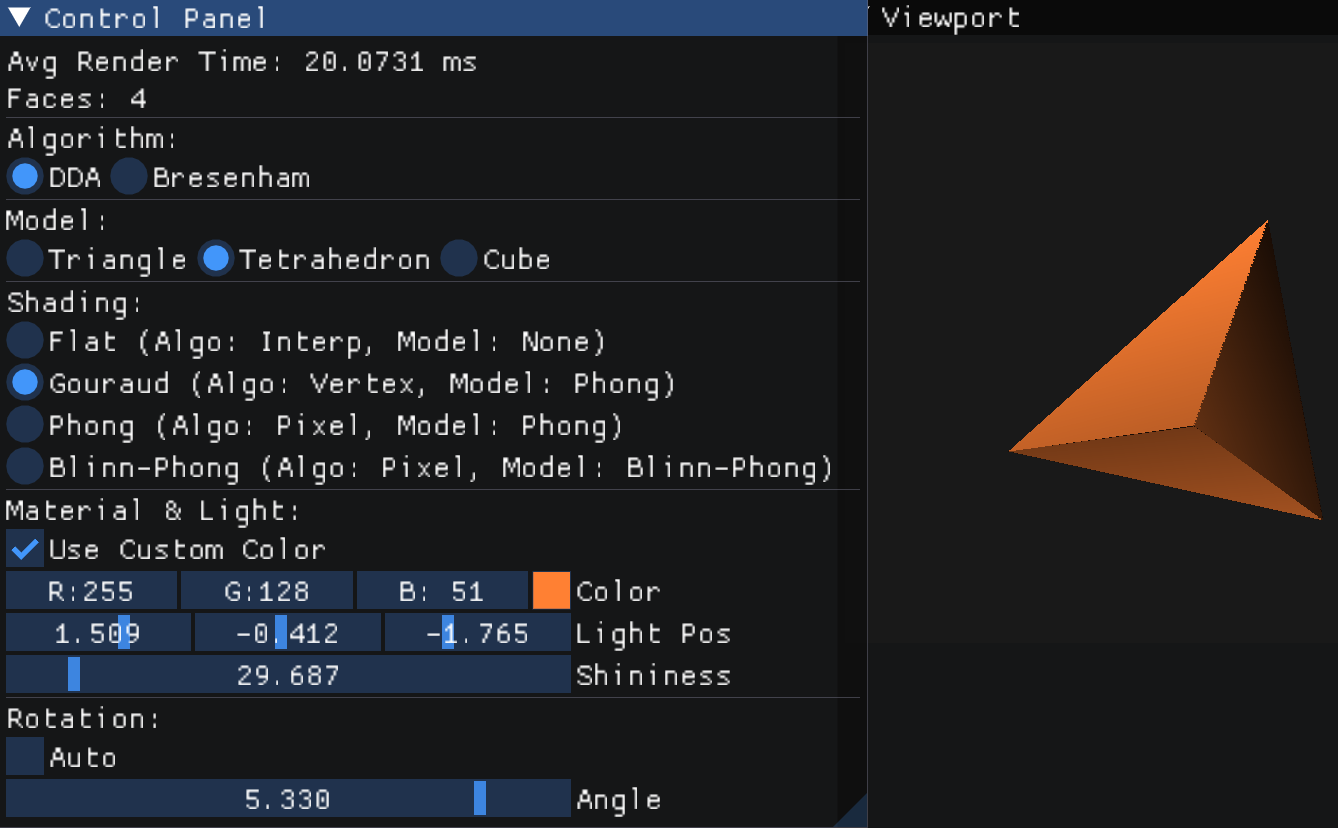
\includegraphics[width=0.65\textwidth]{img/tetra_gouraud.png}
    \caption{Gouraud Shading (正四面体)}
\end{figure}

\begin{figure}[H]
    \centering
    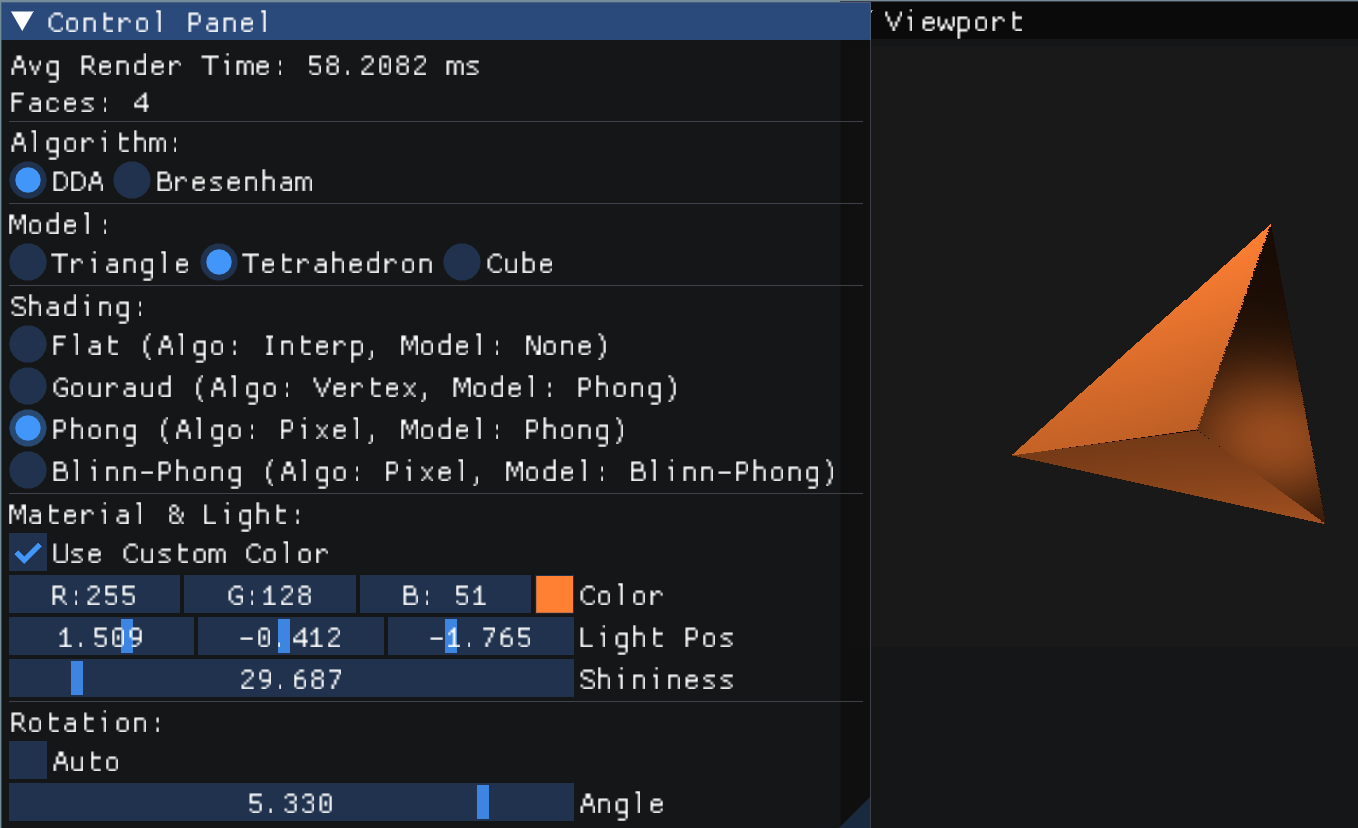
\includegraphics[width=0.65\textwidth]{img/tetra_phong.png}
    \caption{Phong Shading (正四面体)}
\end{figure}

\begin{figure}[H]
    \centering
    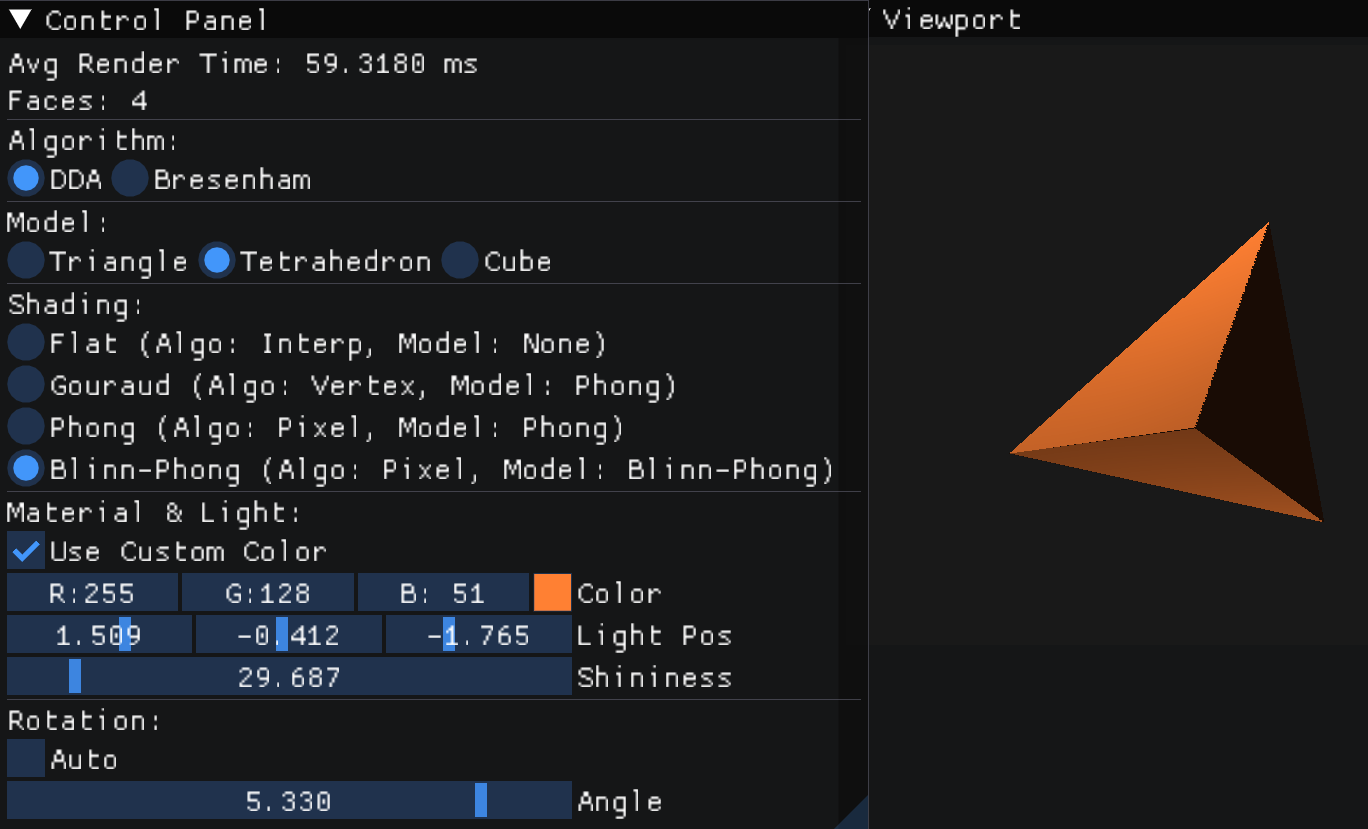
\includegraphics[width=0.65\textwidth]{img/tetra_blinn.png}
    \caption{Blinn-Phong Shading (正四面体)}
\end{figure}

\textbf{第二组：正方体光照效果对比}

\begin{figure}[H]
    \centering
    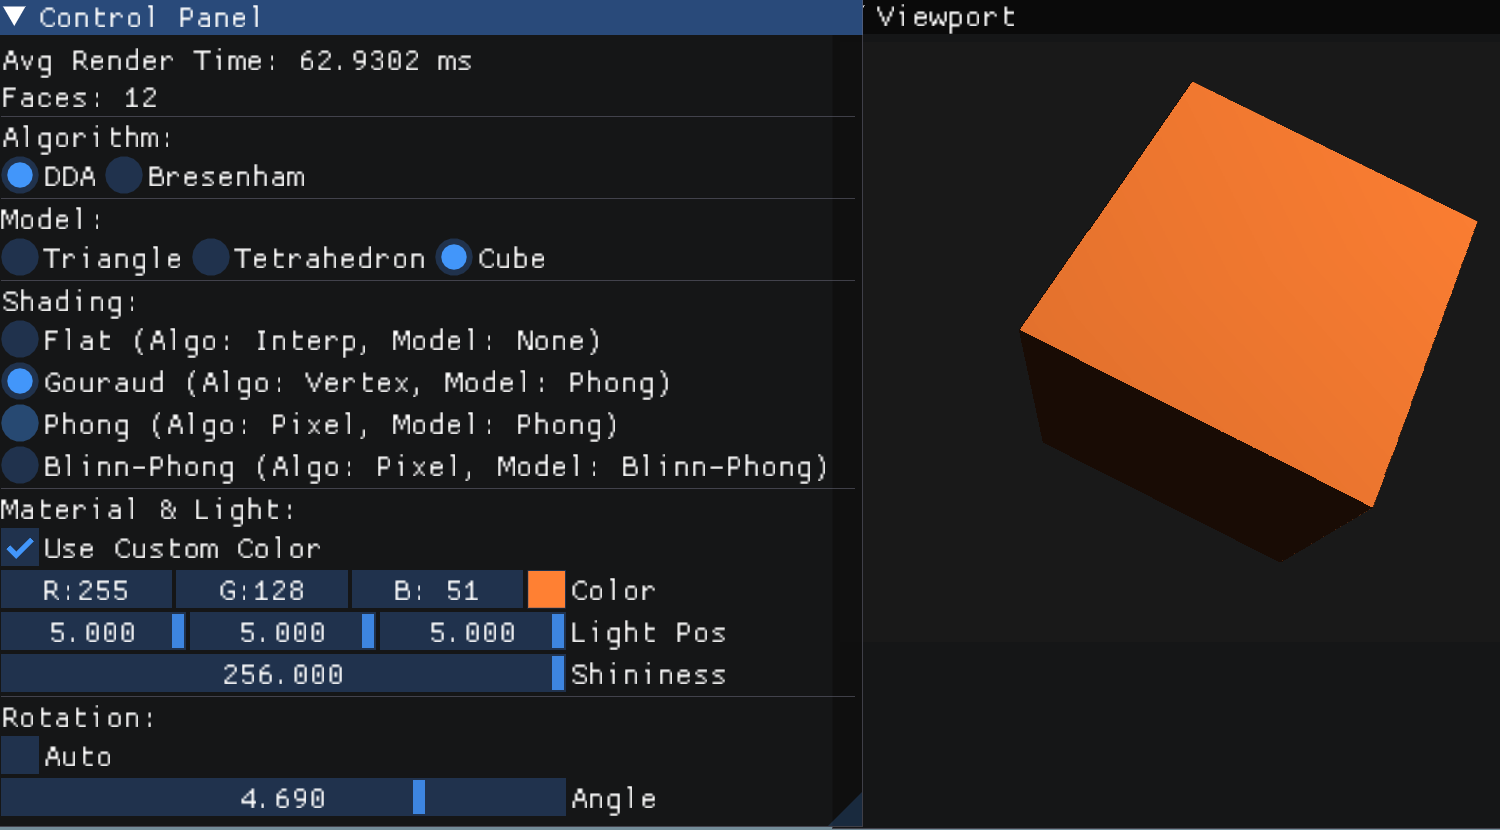
\includegraphics[width=0.65\textwidth]{img/cube_gouraud.png}
    \caption{Gouraud Shading (正方体)}
\end{figure}

\begin{figure}[H]
    \centering
    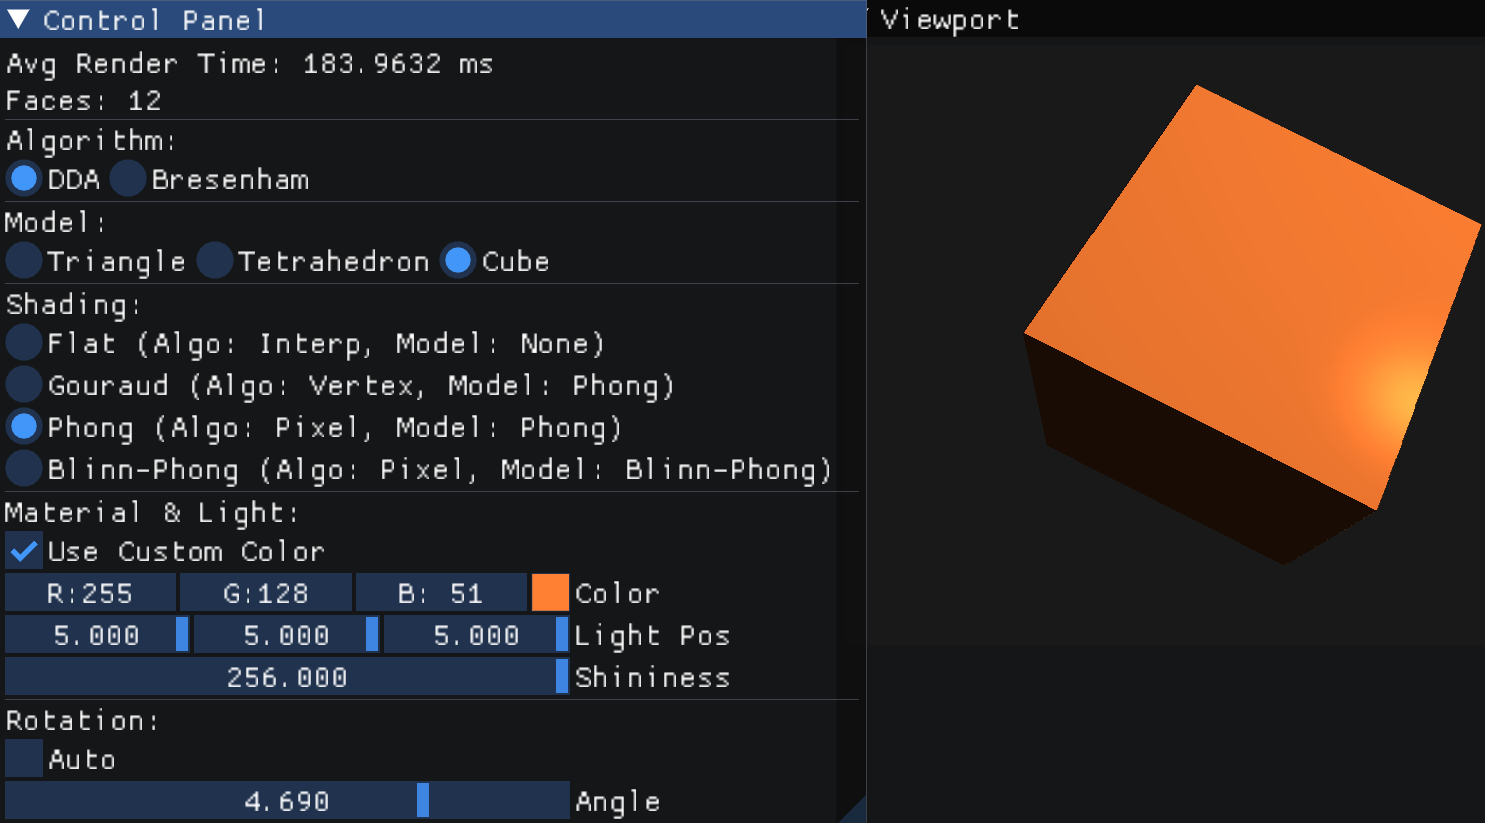
\includegraphics[width=0.65\textwidth]{img/cube_phong.png}
    \caption{Phong Shading (正方体)}
\end{figure}

\begin{figure}[H]
    \centering
    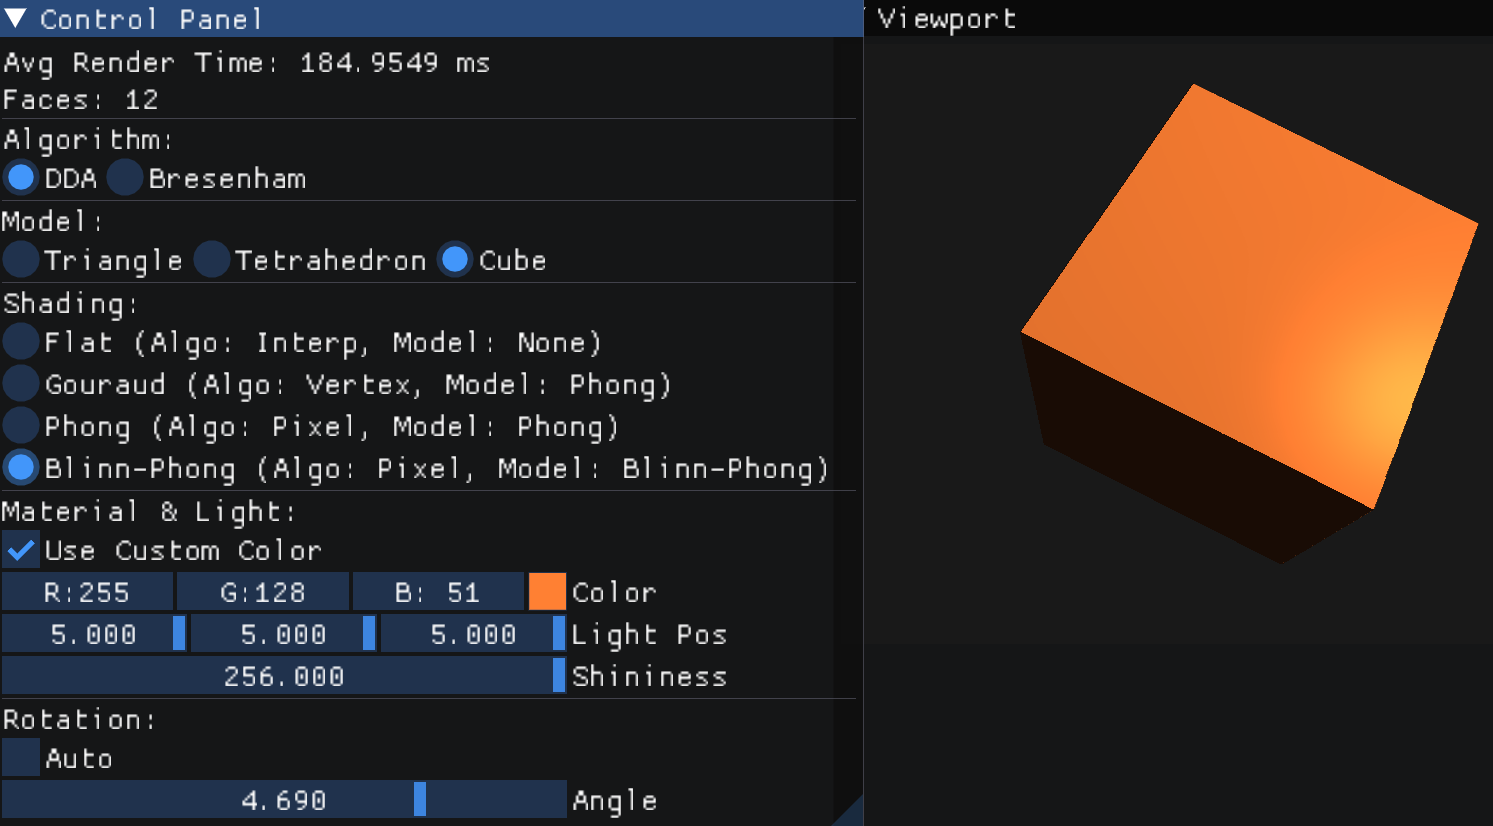
\includegraphics[width=0.65\textwidth]{img/cube_blinn.png}
    \caption{Blinn-Phong Shading (正方体)}
\end{figure}

\subsection{结果分析与讨论}

\subsubsection{光照参数解析}
实验中各项光照参数的物理含义如下：
\begin{itemize}
    \item \textbf{Light Pos (光源位置)}：这也就是代码中的 \texttt{lightPos}，可以调整光线向量 $\vec{L}$ 的方向。
    \begin{itemize}
        \item 在漫反射计算 $max(\vec{N} \cdot \vec{L}, 0)$ 中，光源位置决定了物体表面的明暗分布。
        \item 在镜面反射计算中，光源位置直接决定了高光（Specular Highlight）出现在物体表面的哪个位置。
    \end{itemize}
    \item \textbf{Shininess (反光度/高光系数)}：这就是代码中的 \texttt{shininess}，即光照计算公式中幂运算的指数项。
    \begin{itemize}
        \item 如图中设置 \texttt{Shininess} 约为 30 时，高光光斑较大且边缘发散，模拟塑料或橡胶等粗糙表面的质感。
        \item 当 \texttt{Shininess} 调至最大值 256 时，高光光斑极小且锐利，模拟抛光金属等光滑表面的质感。
    \end{itemize}
    \item \textbf{Color (材质颜色)}：这就是代码中的 \texttt{objectColor}。它与环境光和漫反射光相乘，可以得到物体呈现的基础色调（如截图中的橙色 RGB: 255, 128, 51）。
\end{itemize}

\subsubsection{着色算法效果对比}
通过对比上述六张实验结果图，可以观察到三种算法在处理光照时的显著差异：

\begin{itemize}
    \item \textbf{Gouraud Shading 的高光丢失问题}：
    在正四面体（Tetrahedron）的实验组中，Gouraud 算法的缺陷尤为明显。
    \begin{itemize}
        \item \textbf{现象}：当光源位于三角形面的正前方时，Phong 和 Blinn-Phong 都能在面中心显示出明亮的高光，但 Gouraud 渲染出的面却显得平淡，高光完全消失或极其微弱。
        \item \textbf{原因}：Gouraud 是\textbf{逐顶点}计算光照的。对于正四面体的大三角形面，其三个顶点距离光源较远（或法线夹角较大），计算出的顶点光照强度较低。光栅化阶段对这三个较暗的颜色进行线性插值，导致面中心原本应该最亮的地方反而无法呈现高光。这验证了 Gouraud 着色严重依赖网格密度，无法处理低多边形模型内部的高光。
    \end{itemize}

    \item \textbf{Phong和Blinn-Phong 的高光形态}：
    两者都是\textbf{逐片元}计算，因此都能完美解决 Gouraud 的高光丢失问题，但在高光形态上略有不同：
    \begin{itemize}
        \item \textbf{Phong}：基于反射向量 $\vec{R}$ 和视线 $\vec{V}$ 的夹角。高光通常呈现又亮又小的集中高光，边界较为清晰，与边缘对比明显。
        \item \textbf{Blinn-Phong}：基于法线 $\vec{N}$ 和半程向量 $\vec{H}$ 的夹角。高光形状在某些角度下会略微拉长而呈椭圆状，且边缘过渡比 Phong 稍柔和。在视线与光源夹角较大时能提供更符合物理规律的渐变。
    \end{itemize}
\end{itemize}

\subsubsection{算法效率分析}

\textbf{时间统计机制}
本实验的性能统计是通过 \texttt{glfwGetTime()} 实现的。
\begin{lstlisting}
double startTime = glfwGetTime();
// ... 光栅化循环 (遍历所有三角形) ...
double endTime = glfwGetTime();
// 计算单帧耗时并累积
double frameTime = (endTime - startTime) * 1000.0;
\end{lstlisting}
我记录了每一帧仅包含光栅化和着色计算的核心耗时，排除了 ImGui 界面绘制和 OpenGL 缓冲区交换（SwapBuffers）的时间。通过累计 3 秒内的总耗时除以帧数，得到了较为稳定可见的 \texttt{Avg Render Time}。

\textbf{DDA和Bresenham 绘制效率讨论}

针对单一三角形模型，渲染时间数据是通过\textbf{五次独立运行统计}，每次均在程序自动旋转、界面无其他干扰的情况下，记录 3 秒区间内的平均帧渲染时间，最后取五次结果的算术平均值以消除偶然波动。原始数据如下（均保留四位小数）：

\begin{table}[H]
    \centering
    \begin{tabular}{ccc}
        \toprule
        \textbf{算法} & \textbf{五次统计值 (ms)} & \textbf{平均值 (ms)} \\
        \midrule
        DDA & 6.8137,\ 7.6242,\ 5.7421,\ 6.6589,\ 6.7867 & 6.7251 \\
        Bresenham & 6.5042,\ 6.4781,\ 7.4135,\ 6.4628,\ 6.4083 & 6.6534 \\
        \bottomrule
    \end{tabular}
    \caption{DDA与Bresenham算法效率对比（五次统计取平均）}
\end{table}

\begin{itemize}
    \item \textbf{数据分析}：实验数据显示 Bresenham 算法 (6.65ms) 略快于 DDA 算法 (6.73ms)，性能提升约 1\%。
    \item \textbf{原因讨论}：尽管现代 CPU 浮点性能强大，但在大量边缘步进计算中，Bresenham 的纯整数运算逻辑仍然体现出了微弱的优势。不过，由于光栅化的主要瓶颈在于片元填充（内存写入和深度测试），这种边缘计算的差异在整体渲染时间中占比并不大。
\end{itemize}

\textbf{三种着色模型渲染效率讨论}

同样的，着色模型的效率数据也是\textbf{每种模型和着色模式下分别运行五次}，每次统计 3 秒区间的平均帧渲染时间，最后取平均值。原始数据如下（均保留四位小数）：

\begin{table}[H]
    \centering
    \begin{tabular}{ccccc}
        \toprule
        \textbf{模型} & \textbf{模式} & \textbf{五次统计值 (ms)} & \textbf{平均值 (ms)} \\
        \midrule
        正四面体 & Gouraud & 21.1032,\ 20.3247,\ 19.4018,\ 20.3386,\ 20.1947 & 20.2726 \\
        正四面体 & Phong & 60.6031,\ 59.4278,\ 56.5172,\ 57.4916,\ 58.4417 & 58.4963 \\
        正四面体 & Blinn-Phong & 62.3082,\ 60.2294,\ 61.1837,\ 61.2579,\ 61.2323 & 61.2423 \\
        正方体 & Gouraud & 63.1028,\ 61.3241,\ 59.4197,\ 60.2936,\ 57.1313 & 60.2543 \\
        正方体 & Phong & 188.3087,\ 186.1092,\ 183.2583,\ 185.2016,\ 184.1157 & 185.3987 \\
        正方体 & Blinn-Phong & 183.4096,\ 183.3098,\ 184.3572,\ 185.3625,\ 186.3819 & 184.5642 \\
        \bottomrule
    \end{tabular}
    \caption{不同模型与着色算法的渲染耗时对比（五次统计取平均）}
\end{table}

\begin{itemize}
    \item \textbf{Gouraud对比Phong/Blinn}：
    数据显示 Gouraud 着色的效率显著高于后两者。例如在正方体渲染中，Gouraud 耗时约 60ms，而 Phong/Blinn 均超过 180ms，\textbf{速度相差约 3 倍}。
    这是因为 Gouraud 仅在顶点处计算光照（正方体仅8个顶点或24个独立顶点），而 Phong/Blinn 需要在屏幕上覆盖的每一个像素点进行复杂的向量运算（归一化、点积、幂运算）。

    \item \textbf{Phong对比Blinn-Phong}：
    两者性能非常接近。在正四面体中 Blinn 略慢，在正方体中 Blinn 略快。查询相关资料，可以分析猜测，Blinn-Phong 使用半程向量 $\vec{H}$ 避免了反射向量 $\vec{R}$ 的计算，但在软件光栅化实现中，开方运算（归一化）和幂运算的开销占主导，导致两者差异不明显。

    \item \textbf{模型复杂度影响}：
    从正四面体（4面）到正方体（12面），面数增加了 3 倍。观察数据，Gouraud 时间从 20ms 增至 60ms，Phong 时间从 58ms 增至 185ms，均呈现出\textbf{约 3 倍的线性增长}。这符合查阅资料得到的光栅化渲染的特性：在屏幕覆盖面积相似或几何处理量成比例增加时，渲染耗时与图元数量呈正相关。
\end{itemize}

\section{实验总结}

\subsection{完成情况}
本次实验完成了作业要求的所有基础任务及全部的选做任务：
\begin{enumerate}
    \item \textbf{光栅化算法}：成功实现了 DDA 和 Bresenham 两种三角形边缘生成算法，并结合 Edge-Walking 算法实现了三角形的扫描线填充。
    \item \textbf{着色模型}：完整实现了 Gouraud（逐顶点）、Phong（逐片元）和 Blinn-Phong（逐片元）三种光照着色模型。
    \item \textbf{交互与展示}：构建了完善的 GUI 界面，支持实时切换算法、模型（三角形、四面体、正方体）、着色模式，以及动态调节光源位置、材质颜色和高光系数。
    \item \textbf{性能分析}：针对不同算法和模型进行了详细的帧率统计和效率分析，验证了理论预期。
\end{enumerate}

\subsection{疑难与解决}

\subsubsection{Bresenham 绘制出现的黑线问题}
\textbf{现象}：在使用 Bresenham 算法渲染封闭模型（如正方体）时，偶尔会观察到三角形接缝处出现黑线（漏出背景色）。
\textbf{分析解决}：
\begin{itemize}
    \item \textbf{整数坐标的量化误差（Quantization Error）}：Bresenham 算法本质上是在整数网格上逼近直线。将浮点顶点坐标转换为整数进行边缘计算时发生的截断或取整，导致边缘位置发生微小偏移。这种“对齐到像素中心”的过程会导致边缘位置不够精确。
    \item \textbf{Edge Walking 的精度丢失}：本实验中 Bresenham 用于计算扫描线的左右端点。如果整数步进导致左边界右偏或右边界左偏，就会在原本相连的区域中间留下空隙，透出背景色。
\end{itemize}

\subsubsection{坐标空间的统一}
\textbf{问题}：在初期实现光照计算时，光照效果随视角移动产生异常旋转。
\textbf{分析解决}：检查代码发现是因为光照计算混合了不同空间的坐标。最终统一在\textbf{世界空间（World Space）}进行计算：将顶点位置乘以 Model 矩阵变换到世界空间，法向量使用 Model 的逆转置矩阵变换，光源和相机位置也定义在世界空间。

\subsubsection{深度缓冲的精度}
\textbf{问题}：在物体前后遮挡关系复杂时，出现Z-Fighting（闪烁）现象。
\textbf{分析解决}：确保深度缓冲区 `depthBuffer` 初始化为 1.0f（最大深度），并在 `SetPixel` 中进行严格的 `z < depthBuffer[index]` 测试。同时，在透视投影设置中，将近裁剪面 `near` 设为 0.1f 而非 0.0f，以提高深度缓冲的精度分布。

\subsection{结论与收获}
通过本次实验，我对图形渲染管线的底层原理有了一定的理解：
\begin{itemize}
    \item \textbf{光栅化的本质}：光栅化是将连续的几何数据离散化为像素的过程。DDA 和 Bresenham 虽然在画线算法上有所不同，但在填充三角形时，主要的计算开销在于扫描线内部的属性插值和片元操作，因此两者总体性能差异并不明显。
    \item \textbf{着色频率的重要性}：Gouraud 着色虽然计算效率极高，但其线性插值的特性导致了高光丢失等严重的视觉伪影。Phong 和 Blinn-Phong 通过逐片元计算法线和光照，虽然牺牲了部分性能，但换来了真实细腻的高光效果。质量与效率不可兼得，我们需要权衡。
    \item \textbf{数学基础的应用}：在实现光照模型时，应用了向量点积（计算夹角余弦）、叉积（计算面法线）、归一化等线性代数知识，理解了半程向量 $\vec{H}$ 对镜面反射计算的优化原理，可见数学知识在图形学中的重要性，本人相关方面仍需提高。
\end{itemize}


\end{document}